

\documentclass[a4paper]{article}
\usepackage{Sweave}
\bibliographystyle{plain}



\usepackage{float}


\begin{document}
\Sconcordance{concordance:temptestPlot.tex:temptestPlot.Rnw:%
1 15 1 1 5 6 1 1 2 1 0 5 1 4 0 1 2 6 1 1 2 1 0 11 1 1 3 1 0 5 1 1 2 1 0 %
1 1 1 2 1 0 1 2 7 1 1 2 2 1 6 0 1 4 12 1}







\section{Touching circles lattices }

\begin{center}
\begin{figure}[H]
\begin{Schunk}
\begin{Sinput}
> m<- 3; n<-5;
> hd <- vanItersonTriplePoint(m,n)
> Rise <- hd[1];
> Divergence <- hd[2]
> PG.triple <- newPhyllotaxisGenetic(Rise=Rise,Divergence=Divergence,Jugacy=1,L=2,origin=c(0,-.8))
> plotPhyllotaxis(PG.triple,doCircles=TRUE,plotPrincipals=TRUE,doRepeat=TRUE,doNumbers=TRUE)
\end{Sinput}
\end{Schunk}
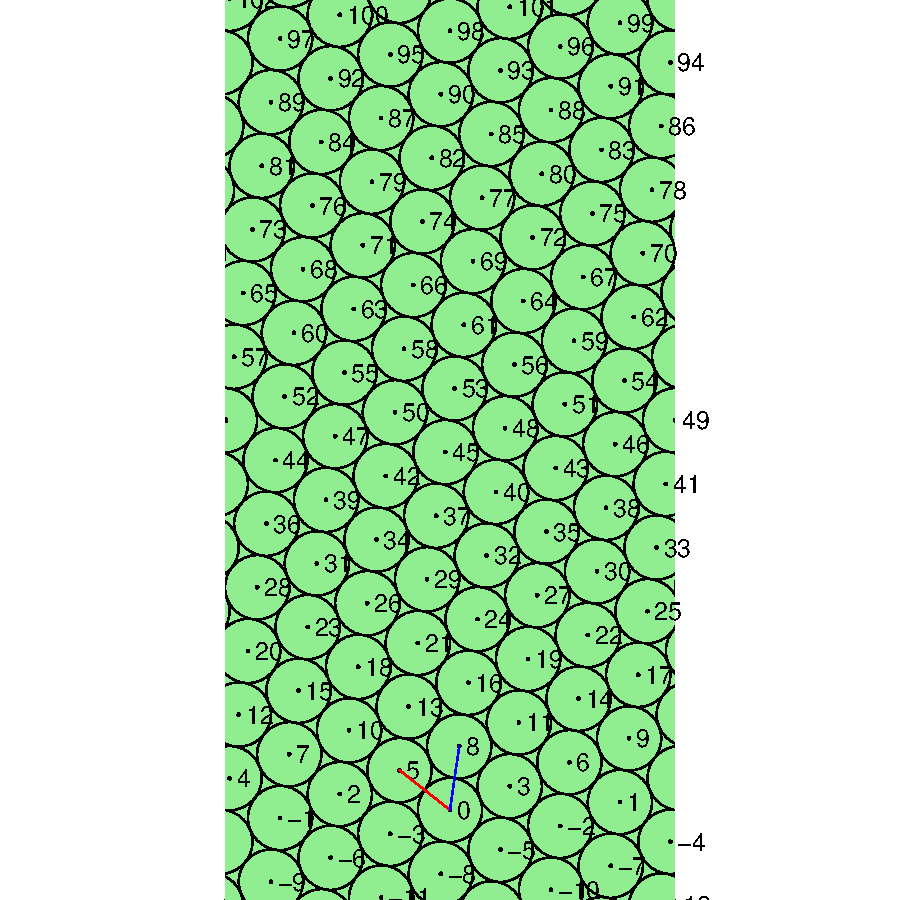
\includegraphics{figdir/cp-plotPGxt}
\caption{A touching circle lattice}
\end{figure}
\end{center}


\begin{center}
\begin{figure}[H]
\begin{Schunk}
\begin{Sinput}
> m<- 3; n<-5;
> hd <- vanItersonTriplePoint(m,n);
> d <- hd[2] + .01
> h <- hvanIterson(m,n,d)
> Rise <- h;
> Divergence <- d
> L <- 2
> PG.38 <-  newPhyllotaxisGenetic(Rise=Rise,Divergence=Divergence,Jugacy=1,L=1.5,origin=c(-1/2+.001,-1))
> PM <- GeometricalPhyllotaxis:::GPPrincipalPhyllotaxisMatrix(PG.38)
> P1 <- GeometricalPhyllotaxis:::getParastichyVector(PM,1)
> P2 <- GeometricalPhyllotaxis:::getParastichyVector(PM,2)
> radius <- sqrt(sum(P1^2))/2
> #windows()
> grid.newpage()
> pushViewport(plotViewport(c(2,2,2,2)))
> pushViewport(dataViewport(xData = c(0,L),yData = c(-L/2,L/2),name="plotRegion"))
> grid.xaxis();
> grid.rect(x=0,width=1,y=0,height=L,default.units="native",just="left",gp=gpar(fill="lightgreen",lty=0))
> circlesWanted <- c(-2,0,1,3,5,6,15)
> #circlesWanted <- seq(from=-2,to=15)
> circles.x <- (circlesWanted * Divergence) %%  1
> .tod <- function(x){ifelse(x>1/2,x-1,x)}
> #circles.x <- .tod(circles.x)
> circles.y <- circlesWanted * Rise
> circlesWanted.left <- c(5)
> circles.x.left <-  ((circlesWanted.left * Divergence) %%  1 ) -1
> circles.y.left <-  circlesWanted.left * Rise
> circlesWanted.right <- c(0,3)
> circles.x.right <-  ((circlesWanted.right * Divergence) %%  1 ) +1
> circles.y.right <-  circlesWanted.right * Rise
> circles.x <- c(circles.x,circles.x.left,circles.x.right)
> circles.y <- c(circles.y,circles.y.left,circles.y.right)
> grid.circle(x=circles.x,y=circles.y,r=radius,default.units="native")
> grid.lines(x=c(0,n*P1[1]),y=c(0,n*P1[2]),default.units="native")
> grid.lines(x=1+c(0,m*P2[1]),y=c(0,m*P2[2]),default.units="native")
> 
> 
\end{Sinput}
\end{Schunk}
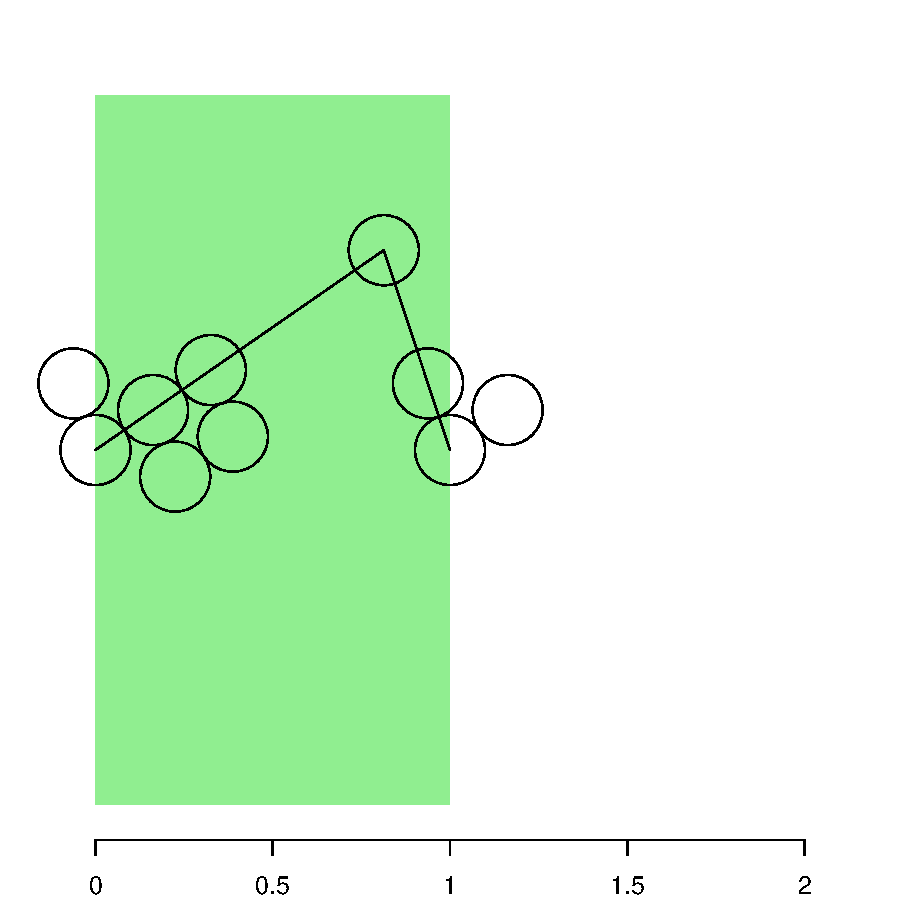
\includegraphics{figdir/cp-plotPGxt2}
\caption{A vesrion of Eickson 3.8}
\end{figure}
\end{center}







%\bibliography{js229}
\end{document}

